%
%   Technische Dokumentation für die Semesterarbeit
%
%   Created by Roman Wuersch on 2010-12-23.	
%
% =============================================================================
% Documentdefinition  beginns here
% =============================================================================

\documentclass[abstracton, listof=totocnumbered,
bibliography=totocnumbered]{scrreprt}
% \documentclass[listof=totoc,bibliography=totoc]{scrreprt}
\usepackage[ngerman]{babel}

\usepackage{tocbasic}

% Use utf-8 encoding for foreign characters
\usepackage[utf8]{inputenc}
% \usepackage[applemac]{inputenc}

% Setup for fullpage use
\usepackage{fullpage}

% Silbentrennung kann unterdrückt werden
\usepackage{hyphenat}

% Tradmark
\def\TTra{\textsuperscript{\texttrademark}}

% Running Headers and footers
%\usepackage{fancyhdr}

% Multipart figures
%\usepackage{subfigure}

% More symbols
%\usepackage{amsmath}
%\usepackage{amssymb}
%\usepackage{latexsym}

% Surround parts of graphics with box
\usepackage{boxedminipage}

% Package for including code in the document
\usepackage{listings}

% If you want to generate a toc for each chapter (use with book)
\usepackage{minitoc}

% Abkürzungsverzeichnis erstellen.
\usepackage[printonlyused]{acronym}

% schöne Tabelle zeichnen
\usepackage{booktabs}
\renewcommand{\arraystretch}{1.2} %Die Zeilenabstände in Tabllen angepasst.

% für variable Breiten
\usepackage{tabularx}

% Durchgestrichener Text
\usepackage[normalem]{ulem} %emphasize weiterhin kursiv

% This is now the recommended way for checking for PDFLaTeX:
\usepackage{ifpdf}

\usepackage[hyperfootnotes=false]{hyperref}
\hypersetup{
  bookmarks=true,         % show bookmarks bar?
  unicode=true,           % non-Latin characters in Acrobat’s bookmarks
  pdftoolbar=true,        % show Acrobat’s toolbar?
  pdfmenubar=true,        % show Acrobat’s menu?
  pdffitwindow=true,      % window fit to page when opened
  pdfstartview={FitH},    % fits the width of the page to the window
  pdftitle={Semesterarbeit},   
  pdfauthor={Roman Würsch},
  pdfsubject={Client-Server-Kommunikation mit Android},
  pdfcreator={TeXnicCenter 1.0 RC1},
  pdfproducer={MiKTeX 2.9},
  pdfnewwindow=true,      % links in new window
  colorlinks=false,       % false: boxed links; true: colored links
  linkcolor=red,          % color of internal links
  citecolor=green,        % color of links to bibliography
  filecolor=magenta,      % color of file links
  urlcolor=cyan          % color of external links
}

\ifpdf
    \usepackage[pdftex]{graphicx}
\else
    \usepackage{graphicx}
\fi

\title{Client-Server-Kommunikation mit Android}

\author{Studierender - Roman Würsch\\
	Projektbetreuer - Beat Seeliger\\
	\\
	HSZ-T - Technische Hochschule Zürich}

\date{Dezember 2010 bis März 2011}

% =============================================================================
% Documenttext beginns here
% =============================================================================

\begin{document}

  \ifpdf
    \DeclareGraphicsExtensions{.pdf, .jpg, .tif}
  \else
    \DeclareGraphicsExtensions{.eps, .jpg}
  \fi
  
  % ===========================================================================
  % Titelblatt beginns here
  % ===========================================================================
  
  \maketitle
  
  % ===========================================================================
  % Abstract beginns here
  % ===========================================================================
  
  \pagenumbering{Alph}
  
  \begin{abstract}
    In dieser Semesterarbeit wird untersucht, wie eine Kommunikation zwischen
    dem Android Betriebsystem und einem Serversystem funktioniert. Es wird
    anhand der plattformunabhängigen Kommunikationsprotokolle REST und Hessian
    ein Prototyp implementiert, der eine grundlegende Funktionalität bietet. Der
    Prototyp soll soweit ausgereift sein, damit man in der Praxis auf ihn
    aufbauen könnte.
    Zudem werden diese beiden Protokolle in einer Gegenüberstellung verglichen.
  \end{abstract}
  
  % ===========================================================================
  % Inahltsverzeichnis beginns here
  % ===========================================================================

  \pagenumbering{Roman}
  
  \tableofcontents
  
  \clearpage
  
  \pagenumbering{arabic}
  
  
  % ===========================================================================
  % Kapitel Administratives beginns here
  % ===========================================================================
  
  \chapter{Personalienblatt}
  \begin{tabbing}
    \hspace*{6cm}\= \kill
    Name, Vorname: \> {\bf Roman Würsch} \\
    Adresse: \> {\bf Murhaldenweg 16} \\
    PLZ, Wohnort: \> {\bf 8057 Zürich} \\
    \\
    Geburtsdatum: \> {\bf 10.11.1980} \\
    Heimatort: \> {\bf Emmetten NW} \\
  \end{tabbing}
  Ich bestätige, dass die vorliegende Semesterarbeit
  ``Client-Server-Kommunikation mit Android'' in allen Teilen selbständig
  erarbeitet und durchgeführt wurde.
  \\
  \\
  \\
  \\
  \\
  \begin{tabbing}
    \hspace*{6cm}\= \kill
    Ort und Datum \> {Unterschrift} \\
  \end{tabbing}
  
  \newpage
  
  
  \newpage
  
  \chapter{Aufgabenstellung}
  
  \section{Ausgangslage}
  Die App-Stores der Mobil-Hersteller boomen. Die Art und Weise wie man Apps
  programmieren soll wird von den Mobil-Hersteller meist klar vorgegeben.
  Sobald jedoch eine App mit einem Server im Internet kommunizieren soll, gibt
  es keine Vorschriften zur Implementierung.
  
  \section{Ziel der Arbeit}
  Es soll eine Client-Server-Kommunikation am Beispiel des Android
  Betriebsystems gezeigt werden. Das Android Betriebsystem nimmt den
  Platz des Clients ein. Als Server wird ein Java EE Applikationsserver
  verwendet.\newline
  
  Folgende Ziele sollen erreicht werden:
  
  \begin{itemize}
    \item Es sollen zwei gängige plattformunabhängigen Arten von
          Daten-Kommunikation miteinander verglichen werden.
    \item Es solle eine detaillierte Anforderungsanalyse an einen
          Prototypen durchgeführt werden.
    \item Es soll ein Prototyp für Daten-Kommunikation implementiert
          werden. Der Prototyp soll beim Server Daten lesen, erstellen,
          aktualisieren und löschen können. Der Prototyp soll auf einem
          Android-Gerät lauffähig sein.
  \end{itemize}
  
  Folgende Punkte werden abgegrenzt, da es den Rahmen der Arbeit sprengen 
  würde:
  
  \begin{itemize}
    \item Der Vergleich der Daten-Kommunikation soll auf zwei Protokolle
          beschränkt werden, die in der Praxis eingesetzt werden,
          \ac{REST}\footnote[1]{
            Der Begriff Representational State Transfer (mit dem Akronym
            REST) bezeichnet einen Softwarearchitekturstil für verteilte
            Hypermedia-Informationssysteme wie das World Wide Web} und
          Hessian\footnote[2]{
            Hessian ist ein binäres Netzwerkprotokoll, mit
            dessen Hilfe Daten zwischen Systemen ausgetauscht und Remote
            Procedure Calls durchgeführt werden können.}.
    \item Der Prototyp des Clients wird für die Android Version 2.2
          (Froyo\footnote[3]{
            Die Android Entwickler geben den verschiedenen Versionen
            ihres Betriebsystems jeweils Namen von süssen Speisen FroYo
            ist ein Akronym für Frozen yogurt}) entwickelt und soll mit dem
          Protokoll \ac{REST}\footnotemark[1] und Hessian\footnotemark[2]
          implementiert werden.
    \item Es werden keine Umfragen, Erhebungen und Feldstudien
          durchgeführt.
  \end{itemize}
  
  \newpage
  
  \section{Aufgabenstellung}
  
  \begin{itemize}
    \item Gegenüberstellung der beiden Protokollkonzepte
    \item Gegenüberstellung der Einsatzgebiete der beiden Protokolle
    \item Prüfen ob eine Implementierung für Android möglich ist
    \item Testszenarien für die beiden Prototypen ausarbeiten
    \item Entwicklung eines Prototypen für beide Protokolle \ac{REST} und
          Hessian
    \item Durchführen der definierten Tests der beiden Prototypen
  \end{itemize}
  
  \section{Erwartete Resultate}
  Die erwarteten Resultate ergeben sich aus der Aufgabenstellung:
  
  \begin{enumerate}
    \item Es wird die Versionskontrolle auf der Basis von GIT bei
          Github.com verwendet.
    \item Planung, Arbeitsnachweis und weitere Informationen werden im WIKI
          von Github.com geführt.
    \item Technischer Bericht
    \begin{enumerate}
      \item Beschreibung der Ausgangslage
      \item Konzeptionelle Gegenüberstellung von \ac{REST} und Hessian
      \item \sout{Gegenüberstellung der Einsatzgebiete von \ac{REST} und
      Hessian}\footnote[4]{
        Im Design-Review hat man sich auf den Verzicht dieses Kapitels
        geeinigt.}
      \item Definition der Anforderungen an den Prototyp 
      \item Ergebnisse der Tests und Abdeckung der Testszenarios
      \item Zusammenfassung zur Entwicklung des Prototypen
    \end{enumerate}
    \item Lauffähiger Prototyp:
    \begin{enumerate}
      \item Es soll ein lauffähiger Prototyp auf der Basis von
            Android 2.2 (Froyo) für beide Protokolle gemacht werden.
      \item Der Prototyp soll bei einem Server Daten lesen, erstellen,
            aktualisieren und löschen können.
    \end{enumerate}
  \end{enumerate}
  
  \newpage  
  
  \chapter{Erreichte Ziele}
  
  Es wurden alle Ziele gemäss den erwarteten Resultaten der Aufgabenstellung
  erreicht.
  
  \begin{enumerate}
    \item \textbf{Erreicht} Die Versionskontrolle liegt öffentlich zugänglich unter der
          Adresse:\\
          \url{https://github.com/sushicutta}
    \item \textbf{Erreicht} Das Wiki ist öffentlich zugänglich unter der
          Adresse:\\
          \url{https://github.com/sushicutta/ClientServerKommunikationMitAndroid/wiki}
    \item \textbf{Noch nicht Erreicht} Technischer Bericht
    \begin{enumerate}
      \item \textbf{Erreicht} Beschreibung der Ausgangslage
      \item \textbf{Erreicht} Konzeptionelle Gegenüberstellung von \ac{REST} und
            Hessian
      \item \textbf{Erreicht} Dieses Ziel wurde beim Design-Review gestrichen. 
      \item \textbf{Erreicht} Definition der Anforderungen an den Prototyp
      \item \textbf{Erreicht} Ergebnisse der Tests und Abdeckung der Testszenarios
      \item \textbf{Noch nicht Erreicht} Zusammenfassung zur Entwicklung des
            Prototypen
    \end{enumerate}
    \item \textbf{Erreicht} Lauffähiger Prototyp:
    \begin{enumerate}
      \item \textbf{Erreicht} Der Sourcecode für den lauffähigen Prototypen des
      Clients ist öffentlich zugänglich unter folgender Adresse, der gültige Branch
      heisst: restWithGlassFish\\
      \url{https://github.com/sushicutta/ClientServerKommunikationMitAndroid}
      \item \textbf{Erreicht} Der Sourcecode für den lauffähigen Prototypen des
      Servers ist öffentlich zugänglich unter folgender Adresse, der gültige Branch
      heisst: jpa\\
      \url{https://github.com/sushicutta/Semesterarbeit}
    \end{enumerate}
  \end{enumerate}
  
  \chapter{Beschreibung der Ausgangslage}
  
  Für das Informatik Diplomstudium an der Fachhochschule Zürich für Technik
  HSZ-T wird von den Studenten verlangt eine Semesterarbeit eigenständig zu
  verfassen.
  
  \section{Wahl des Themas}
  
  Seit dem Siegeszug der Smartphones, welcher durch das iPhone von Apple
  eingeläutet wurde interessiere ich mich für mobile Geräte. Durch das
  Interesse an Linux und an freien und offenen Systemen bin ich bei Android als
  Betriebsystem gelandet. Google versucht mit Android das zu erreichen, was
  Apple mit dem iOS erreicht hat. Sie wollen Entwicklern eine einfach
  Schnittstelle für die Entwicklung neuer Software bieten. Zudem soll die
  Software über einen von Google gesteuerten Marktplatz zur Verfügung gestellt
  werden.
  
  Die Entwicklung neuer Software für Android wird von Google mittels Tutorials
  gefördert. Dabei habe ich persönlich keinen Hinweis auf die Datenkommunikation
  zwischen Android und Fremdsystemen bekommen. Da eine solide
  Datenkommunikation heutzutage zu den Grundbedürfnissen in der
  Softwareentwicklung gehört, wollte ich die Möglichkeit zweier
  systemunabhängigen Methoden näher betrachten.
  
  Bei der Auswahl der beiden Protokolle bin ich schnell auf \ac{REST} gestossen,
  da es sich in den letzten paar Jahren zu einer populären Methode entwickelt
  hatte. Von Hessian als Kommunikationsprotokoll hatte ich nur schon gehört,
  ich wusste aber, dass es für die meisten gängigen Programmiersprachen eine
  Implementierung gibt, somit ist es in den Kreis meiner Auswahl gefallen.
  
  \section{Bewertungskriterien}
  
  Wie im Kick-off Meeting festgelegt, werden die Bewertungskriterien aus dem
  Bachelor Studiengang verwendet. 
  
  \section{Sprache}
  
  Der Bericht wird in deutscher Sprache verfasst. Englische Ausdrücke werden im
  Context verwendet, wenn man davon ausgehen kann, dass es Ausdrücke aus dem
  Gebiet der Informatik sind, die man versteht.
  
  \newpage
  
  \section{Projekt Termine}
  
  Die Projekt Termine wurden alle eingehalten, siehe Tabelle \ref{tab:termine}.
  \newline
  
  \begin{table}[h]
    \begin{center}
      \begin{tabular}{lp{7cm}ll}
        \toprule
        Termin & Datum & Ort \\
        \midrule
        14. 12. 2010 & Kick-off Meeting & Panter GmbH\\
        12. 01. 2011 & Design-Review Meeting & HSZ-T\\
        16. 02. 2011 & Abgabe der Dokumentation & HSZ-T\\
        02. 03. 2011 & Schlusspräsentation & HSZ-T\\
        \bottomrule
      \end{tabular}
      \caption{Projekt Termine}
      \label{tab:termine}
    \end{center}
  \end{table}
  
  \section{Projekt Historie}
  
  In der Projekt Historie sind die wichtigsten Meilensteine ersichtlich, siehe
  Tabelle \ref{tab:projekthistorie}.
  \newline
  
  \begin{table}[h]
    \begin{center}
      \begin{tabular}{lp{9cm}ll}
        \toprule
        Datum & Status & Wer \\
        \midrule
        06. 12. 2010 & Ein Dozierender hat die Arbeit inkl. Aufgabenstellung
        ausgeschrieben und wartet auf einen Studierenden der diese Arbeit
        durchführt & Roman Würsch\\
        07. 12. 2010 & Die Arbeit ist freigegeben & Olaf Stern\\
        14. 12. 2010 & Freigabe Kick-Off & Beat Seeliger\\
        12. 01. 2011 & Freigabe Desgin-Review & Beat Seeliger\\
        16. 02. 2011 & Abgabe der Dokumentation & Roman Würsch\\
        02. 03. 2011 & Präsentation der Arbeit & Roman Würsch\\
        \bottomrule
      \end{tabular}
      \caption{Projekt Historie}
      \label{tab:projekthistorie}
    \end{center}
  \end{table}
  
  \section{Richtlinien}
  Folgende Dokumente mit Richtlinien der Hochschule für Technik Zürich 
  wurden für die Semesterarbeit berücksichtigt:

  \begin{itemize}
      \item Reglement \cite{hsz_reglement}
      \item Ablauf \cite{hsz_ablauf}
      \item Bewertungskriterien \cite{hsz_bewertungskriterien}
  \end{itemize} 
  
  \newpage
  
  \chapter{Konzeptionelle Gegenüberstellung von REST und Hessian}
  
  \section{REST – Representational State Transfer}
  
  \ac{REST} stammt aus der Dissertation von Roy Fielding in der er den Erfolg
  des \ac{WWW} auf bestimmte Eigenschaften der verwendeten Mechanismen und
  Protokolle (z. B. \ac{HTTP}) zurückführt.
  
  \subsection{Was ist REST}
  
  Der Client ändert den Status mit jeder Ressource Repräsentation.
  
  \begin{enumerate}
    \item Ein Client referenziert eine Web Ressource über eine \ac{URL}.
    \item Der Server lieferte eine Repräsentation der Ressource in einer vom
    Client akzeptierten Form, z.B. als ein \ac{HTML} Dokument oder als \ac{XML}.
    \item Die vom Server geladene Ressource versetzt den Client in einen neuen
    Status und bietet evtl. Links zu neuen Ressourcen an.
    \item Der Client lädt eine ihm neue bekannte Ressource über die \ac{URL},
    was wieder in einem Ressource Access endet.
    \item Die vom Server geladene Ressource versetzt den Client wieder in einen
    neuen Status.
  \end{enumerate}
  
  \subsection{Wie funktioniert REST}
  
  \begin{itemize}
    \item \ac{REST} verwendet \ac{URL} um Ressourcen zu adressieren
    \item \ac{REST} verwendet (a) HTTP-PUT, (b) HTTP-GET, (c) HTTP-POST und
    (d) HTTP-DELETE Requests um Daten zu (a) kreieren, (b) lesen,
    (c) aktualisieren und (d) zu löschen.
    \item \ac{REST} verwendet Standard Ressource Repräsentationen wie \ac{HTML},
    \ac{XML}, \ac{JSON}, usw.
    \item \ac{REST} verwendet \ac{HTTP} Header ``Content-type'' wie text/html,
    application/xml, application/json, usw. um die Codierung der Ressourcen zu
    deklarieren.
    \item \ac{REST} liefert die codierten Ressourcen aufgrund des \ac{HTTP} Header
    ``Accept''.
    \item \ac{REST} liefert bei einem Request \ac{HTTP} Statuscodes. 2xx bei einem
    erfolgreichen Request oder 4xx wenn der Request fehlgeschlagen ist. Es
    können auch weitere Statuscodes, wie 3xx oder 5xx, zurückgegeben werden, je
    nach Definition.
  \end{itemize}
  
  \subsection{Wieso REST}
  
  Das \ac{WWW} hat sich in den letzten Jahren bewährt. Das \ac{WWW} ist
  skalierbar und einfach zu verstehen. Wenn die Kommunikation von Maschine zu Mensch
  funktioniert, dann ist sie sicher gut genug um auch von Maschine zu Maschine
  zu funktionieren.
  
  Fast jede Plattform unterstützt die Standards des \ac{WWW}, damit macht es
  eine Plattform übergreifende Kommunikation möglich.
  
  Im \ac{WWW} gibt es Standards für Security (z.B. \ac{HTTPS}) und Caches (z.B.
  \ac{HTTP} ETag), welche mit \ac{REST} verwendet werden können. 
  
  \section{Hessian}
  
  Hessian ist ein leichtgewichtiges Kommunikationsprotokoll, das von Caucho
  Technology, Inc. entwickelt wurde.
  
  \subsection{Was ist Hessian}
  
  Hessian ist ein binäres Netzwerkprotokoll, dass für \ac{RPC} und
  Datenkommunikation zwischen Computersystemen verwendet werden kann. Hessian wird üblicherweise
  über \ac{HTTP} übertragen. Hessian definiert keine \ac{IDL} oder ein externes
  Schema wie man das aus \ac{SOAP} oder \ac{CORBA} kennt. Die Schnittstelle (sprich
  Methoden Interfaces) des Servers muss beim Client bekannt sein.
  
  \subsection{Was beinhaltet Hessian}
  
  Hessian definiert hauptsächlich zwei Dinge.
  
  \begin{enumerate}
    \item Wie ein Remote Procedur Call ausgeführt wird. Dabei wird
    definiert, wie eine Methode auf einem Objekt aufgerufen wird und wie die
    dazugehörigen Argumente übergeben werden. Zudem wird auch definiert wie der
    Reply der Methode aussieht. Zudem werden im Fehlerfall so genannte Faults
    zurückgegeben, was nichts anderes ist als eine Exception.
    \item Die Serialisierung von Daten. Es werden neun primitive zwei
    kombinierte und spezielle Konstrukte unterstützt. Bei den primitiven
    Datentypen handelt es sich um folgende:
    \begin{itemize}
      \item boolean
      \item 32-bit int
      \item 64-bit long
      \item 64-bit double
      \item 64-bit date
      \item UTF8-encoded string
      \item UTF8-encoded xml
      \item raw binary data
      \item remote objects
    \end{itemize}
    Kombinierte Konstrukte sind:
    \begin{itemize}
      \item list für Listen und Arrays
      \item map für Objects und Hashtabellen
    \end{itemize}
    Die speziellen Konstrukte sind:
    \begin{itemize}
      \item null für null values
      \item ref Referenzen auf ein object in einer list oder map
    \end{itemize}
  \end{enumerate}
  
  \subsection{Wieso Hessian}
  
  Als binäres Protokoll ist Hessian insbesondere für die Versendung von
  Binärdaten geeignet. Binäre Protokolle wie RMI und Hessian sind darüber
  hinaus wesentlich performanter als XML basierte Protokolle, wie z.B. \ac{SOAP}
  oder XML-RPC.

  Hessian wurde von den Erfindern für verschieden Programmiersprachen portiert,
  damit macht es eine Plattform übergreifende Kommunikation möglich.
  
  \enlargethispage{3cm}
  
  \section{Gegenüberstellung}
  
  In der Tabelle \ref{tab:gegenueberstellungRestHessian} werden die wichtigsten
  Eigenschaften verglichen.
  \newline
  
  \begin{table}[h]
    \begin{center}
      \begin{tabular}{p{2.4cm}p{6.1cm}p{6.1cm}}
        \toprule
        Aspekt & REST & Hessian \\
        \midrule
        \nohyphens{Standard} & Kein Standard, verwendet existierende Standards wie
        RFC2616 HTTP 1.1 & Kein Standard, wurde von Caucho Technology, Inc entwickelt\\
        \cmidrule{2-3}
        \nohyphens{Ressource Adressierung} & Jede Ressource hat ihre eigene \ac{URL}
        & Indirekt über Hessian funktionen\\
        \cmidrule{2-3}
        \nohyphens{URL} & Wird verwendet für die Adressierung der einzelnen
        Ressourcen & Wird für den Hessian Endpoint (Servlet) verwendet\\
        \cmidrule{2-3}
        \nohyphens{Error handling} & Server Statuscodes 4xx und 5xx im Response &
        Hessian Fault\\
        \cmidrule{2-3}
        \nohyphens{Daten Repräsentation} & Alle Encodings von \ac{HTTP} definiert,
        wie (Text, \ac{HTML}, \ac{XML}, \ac{JSON}, usw.) & Serialisierung
        gemäss Hessian Protokoll\\
        \cmidrule{2-3}
        \nohyphens{HTTP} & PUT, GET, POST, DELETE sind auf Funktionen gemappt & POST
        wird für den Transport verwendet\\
        \cmidrule{2-3}
        \nohyphens{State} & Stateless, serverseitig wird nichts gespeichert &
        Stateful, jede Hessian funktion ist ein Teil einer definierten Applikation\\
        \cmidrule{2-3}
        \nohyphens{Interface} & \ac{HTTP} PUT, GET, POST, DELETE & Keine \ac{IDL}
        wie bei \ac{CORBA}, das Interface muss aber bekannt sein.\\
        \cmidrule{2-3}
        \nohyphens{Transaktionen} & Nicht direkt unterstützt, eine Transaktion
        könnte über Ressourcen abgebildet werden. & Transaktion Context kann im Header übergeben
        werden\\
        \bottomrule
      \end{tabular}
      \caption{Gegenüberstellung von REST und Hessian}
      \label{tab:gegenueberstellungRestHessian}
    \end{center}
  \end{table}
  
  \clearpage
 
  \section{Persönliche Meinung}
  
  Da ich mich nun tiefer mit beiden Protokollen beschäftigt habe, möchte ich
  noch meine Meinung dazu abgeben.
  
  \subsection{REST ist ``cool'', aber der Teufel steckt im Detail}
  
  REST ist in aller Munde. Seit gut drei Jahren höre ich immer wieder, wie
  einfach dass eine Schnittstelle mit REST zu implementieren ist. Das mag auch
  sein, wenn man sich an einen Standard wie JSR-000311\cite{JSR311} hält, und
  den Server, wie auch den Client, nach diesem Schema umsetzt. Leider aber sieht
  es schon anders aus, wenn der Server in Ruby on Rails\cite{RoR} geschrieben
  wurde und der Client in Java implementiert wird. Diese Erfahrung habe ich
  gemacht, als ich das im Rahmen der Semesterarbeit versucht habe. Die
  Unterschiede zeigen sich in den Finessen, wie zum Beispiel ein
  HTTP-Responsecode aussieht, wenn ich auf die \ac{URL} einer ehemals
  publizierten Ressource, welche mit Ruby on Rails bereitgestellt wurde,
  zugreife, die aber schon einmal gelöscht wurde. Da kann es durchaus
  vorkommen, dass dann nicht ein Responsecode 404 (Not Found), wie erwartet, 
  sonder ein Responsecode 406 (Not Acceptable) zurückgegeben wird. Zudem kommen
  optionale Headerfelder, die in einem HTTP-Request oder HTTP-Response Objekt verpackt
  werden können, und so weiter. Wie man hier sieht, gibt es viele verschiedene
  Arten, wie man ein RESTful Webservice auslegen kann.
  
  Wenn man demnach versucht eine plattformunabhängige
  Kommunikationsschnittstelle zur Verfügung zu stellen, oder eine solche
  anzubinden, muss man alle möglichen Fälle von Ressourcezugriffen untersuchen,
  und auch deren Fehlerfälle alle korrekt abarbeiten, nur so kann man
  gewährleisten, dass man eine ``coole'' Schnittstelle gebaut hat.
  
  Natürlich gibt es auch die Vorteile, welche nicht vernachlässigt werden
  dürfen. Da sehe ich die weit aus Grössten in der Repräsentation der Daten und
  der Verständlichkeit der einzelnen Zugriffe über einzelne \ac{URL}'s. Hinzu
  kommt, dass namhafte Firmen wie Amazon oder Yahoo bereits Schnittstellen zu
  ihren Systemen über REST bereitstellen, was den Akzeptanzfaktor in einem
  möglichen Projekt enorm erhöht.

  Wie die Schnittstelle eines möglichen Produktservices aussehen würde, möchte
  ich anhand einer Grafik \ref{restPrinzip} zeigen:
  
  \begin{figure}[h]
      \begin{center}
          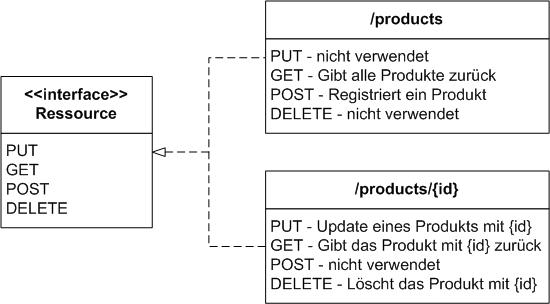
\includegraphics[width=0.7\textwidth]{./image/rest.png}
          \caption{Ein Produktservice mit REST bereitgestellt}
          \label{restPrinzip}
      \end{center}
  \end{figure}
  
  \subsection{Hessian ist leichtgewichtig, aber leider kein Standard}
  
  Ganz nach dem KISS-Prinzip\cite{KISS} wurde dieses Protokoll geschaffen. Es
  soll so einfach wie möglich anzuwenden sein, und das ist es auch. Für den
  Serverteil, reicht ein Interface, und die ausprogrammierte Klasse ist auch
  schon in ein paar Zeilen Code geschrieben. Dann noch die nötige Konfiguration
  für den Servlet-Container. Die ganze Magie, der Methodinvocation und
  Serialisierung der Daten, wird über das Package com.caucho.hessian.*
  abgewickelt, davon sieht man als Softwareentwickler nichts mehr. Der Client
  ist wird wie der Server auch gleich kurzerhand realisiert. Die aktuelle
  Version 4.0.7 ist als JAR File gerade einmal 383 Kilobyte gross und
  beinhaltet alle Klassen um als Server oder als Client zu fungieren. Ein
  Beispiel Code in Java könnte in etwa so aussehen:\\

  Das Interface:
  
\begin{verbatim}
package example;  

public interface Basic {

  public String hello();
  
}
\end{verbatim}

  Die ausprogrammierte Klasse:

\begin{verbatim}
package example;  
  
import com.caucho.hessian.server.HessianServlet;

public class BasicServiceEndpoint extends HessianServlet implements Basic {

  @Override
  public String hello() {
    return "Hello World";
  }
      
}
\end{verbatim}

  Dann fehlt nur noch die Konfiguration für den Servlet-Container im web.xml,
  und schon kann über die \ac{URL} http://www.examplehost.com/BasicService auf
  den Server zugegriffen werden.:
  
\begin{verbatim}
<web-app>  
  <servlet>
    <servlet-name>BasicService</servlet-name>
    <servlet-class>example.BasicServiceEndpoint</servlet-class>
    </servlet>
  <servlet-mapping>
      <servlet-name>BasicService</servlet-name>
      <url-pattern>/BasicService</url-pattern>
  </servlet-mapping>
</web-app>
\end{verbatim}

  Der Client kommt auch schön schlank daher:

\begin{verbatim}  
package example;

import com.caucho.hessian.client.HessianProxyFactory;

public class BasicClient {

  public static void main(String []args) throws Exception {
  
    String url = "http://www.examplehost.com/BasicService";

    HessianProxyFactory factory = new HessianProxyFactory();
    Basic basic = (Basic) factory.create(Basic.class, url);

    System.out.println(basic.hello());
    
  }
  
}
\end{verbatim}  
  
  Als Nachteil sehe ich den geringen Bekanntheitsgrad von Hessian und zudem,
  dass Hessian kein Standard ist. In einem grösseren Entwicklungprojekt, dürfte
  ein Webservice wohl mit \ac{SOAP} oder einer ähnlichen Technik umgesetzt
  werden, da es sich dabei effektiv um einen Standard handelt. Zudem dürfte es
  komplizierter werden, wenn man Datentypen verwendet, die im Protokoll nicht
  für die Serialisierung vorgesehen sind
  
  \subsection{Fazit}
  
  Für kleine Projekte, oder Projekte wo die Grösse des ausgelieferten Packets
  eine Rolle spielen würde ich auf Hessian setzten. Durch die
  Leichtgewichtigkeit und die Einfachheit der Implementierung hat man mit
  Hessian ein mächtiges Werkzeug.
  
  Bei einem Projekt, wo man nicht nur eine Kommunikation von Maschine zu
  Maschine bauen soll, sondern auch eine Schnittstelle für Menschen
  bereitstellt, würde ich auf \ac{REST} setzten. Da man die Repräsentation
  gleich für maschinentaugliche, wie auch für browsertaugliche (was ja von
  Menschen verwendet wird) Formate bereitstellen kann. Sprich, die Ressourcen in
  \ac{XML} und gleich in \ac{HTML} zu präsentrieren, macht da keinen grossen
  Unterschied mehr. Zudem fällt eine Dokumentation der Schnittstelle fast
  komplett weg, oder wenn wirklich nötig, kann die Dokumentation der
  Schnittstelle gleich als eigene Ressource über eine \ac{URL} zugänglich
  gemacht werden.
  
  \newpage
  
  \chapter{Definition der Anforderungen an den Prototyp}
  
  Die Definition der Anforderungen an die Prototypen werden mit der Technik der
  User Sto\-ries\cite{UserStories} gemacht.
  
  \section{Was sind User Stories}
  
  User Stories beschreiben Anforderungen an eine Software in einer für Jedermann
  verständlichen Sprache. Es sollen keine technischen Details genannt, sondern
  viel eher Eigenschaften erläutert werden die jeder versteht. Oft werden User
  Stories als Aktionen in einem \ac{GUI} verfasst. Aus den User Stories kann
  man die jeweiligen Akzeptanztests\cite{AcceptanceTests} ableiten.
  
  Eine User Story sollte nicht mehr als drei Sätze haben. Das kommt daher, dass
  eine User Story nie zu komplex sein darf. Wenn man mehr als drei Sätz für die
  Beschreibung einer User Story braucht, sollte diese in mehrere kleinere User
  Stories aufgeteilt werden, welche genug simpel sind, um wiederum in drei
  Sätzen beschrieben zu werden.
  
  Jeder User Story wird mit einer eindeutigen Nummer versehen: US-\{User Story
  Nummer\}
  
  \section{Anforderungen an den Prototyp}
  
  Im folgenden werden die Anforderungen an den Prototypen spezifziert. Die
  Anforderungen werden aus zwei Blickwinkeln definiert. Aus der Sicht eines
  Anwenders und aus der Sicht eines Informatikstudenten. Diese beiden
  Sichtweisen werde jeweils ich vertreten, da ich mich davon abgegrenzt habe,
  irgenwelche Erhebungen durchzuführen.
  
  Nachfolgend ist die Rede von Datenobjekten. Bei einem Datenobjekt wie es hier
  aufgeführt wird, handelt es sich um ein \ac{POJO}. 
  
  \newpage
  
  \section{Aus der Sicht des Anwenders}
  
  Der Anwender stellt ein Mensch dar, der nur die Sicht auf die
  Clientapplikation hat. Normalerweise hat ein Anwender keinerleit technische
  Hintergründe. Die definierten User Stories aus der Sicht des Anwenders sind in
  der Tabelle \ref{tab:anwenderUserStories} ersichtlich.
  \newline
  
  \begin{table}[h]
    \begin{center}
      \begin{tabular}{cp{13cm}l}
        \toprule
        User Story & Beschreibung \\
        \midrule
        US-1 & Ich als Anwender will ein hochwertiges \ac{GUI}. \\
        US-2 & Ich als Anwender will meine Applikation überall verwenden können. \\
        US-3 & Ich als Anwender will eine stabile Applikation. \\
        US-4 & Ich als Anwender will ein ausgewähltes Datenobjekt vom Server an mein
        Androidgerät übertragen und darstellen können. \\
        US-5 & Ich als Anwender will eine komplette Liste von Datenobjekten vom
        Server an mein Androidgerät übertragen und darstellen können. \\
        US-6 & Ich als Anwender will ein ausgewähltes Datenobjekt auf dem Server
        löschen können. \\
        US-7 & Ich als Anwender will ein ausgewähltes Datenobjekt auf dem Server
        editieren können. \\
        US-8 & Ich als Anwender will ein neues Datenobjekt an den Server übertragen
        können. Dieses Datenobjekt soll für zukünftige Zugriffe auf dem Server
        gespeichert werden. \\
        US-9 & Ich als Anwender will über Übertragungsfehler informiert werden. \\
        \bottomrule
      \end{tabular}
      \caption{User Stories eines Anwenders}
      \label{tab:anwenderUserStories}
    \end{center}
  \end{table}
  
  \newpage
  
  \section{Aus der Sicht des Informatikstudenten}
  
  Der Informatikstudent stellt ein Mensch dar, der sowohl die Sicht auf den
  Client, wie auch auf den Server der Applikation hat. Der Informatikstudent
  versucht durch technische Hilfsmittel die Anforderungen eines Anwenders zu
  erfüllen.
  
  \subsection{Clientapplikation}
  
  Die definierten User Stories zum Client aus der Sicht des Informatikstudent
  sind in der Tabelle \ref{tab:clientUserStories} ersichtlich.
  \newline
  
  \begin{table}[h]
    \begin{center}
      \begin{tabular}{cp{13cm}l}
        \toprule
        User Story & Beschreibung \\
        \midrule
        US-10 & Ich als Informatikstudenten will, dass die Clientapplikation für
        Geräte mit der Android Version 2.2 lauffähig ist. \\
        US-11 & Ich als Informatikstudenten will, dass die Clientapplikation
        unabhängig von der Serverapplikation ausgeliefert werden kann. \\
        \bottomrule
      \end{tabular}
      \caption{User Stories eines Informatikstudenten zum Client}
      \label{tab:clientUserStories}
    \end{center}  
  \end{table}
  
  \subsection{Serverapplikation}
  
  Die definierten User Stories zum Server aus der Sicht des Informatikstudent
  sind in der Tabelle \ref{tab:serverUserStories} ersichtlich.
  \newline
  
  \begin{table}[h]
    \begin{center}
      \begin{tabular}{cp{13cm}l}
        \toprule
        User Story & Beschreibung \\
        \midrule
        US-12 & Ich als Informatikstudent will, dass die Serverapplikation auf
        einem Java EE 6 fähigen GlassFish Applikationsserver läuft. \\
        US-13 & Ich als Informatikstudent will, dass die Serverapplikation sowohl
        Requests über das \ac{REST} Protokoll wie auch über das Hessian
        Protokoll bearbeiten kann. \\
        US-14 & Ich als Informatikstudent will, dass Datenobjekte auf der
        Serverapplikation gespeichert werden können. Diese Daten sollen nur solange
        gespeichert sein, wie der Server läuft. \\
        US-15 & Ich als Informatikstudent will, dass mehrere Clientapplikationen
        gleichzeitig mit der Serverapplikation bedient werden können. \\
        US-16 & Ich als Informatikstudent will, dass die Serverapplikation
        auf dem Internet zugänglich ist. \\
        US-17 & Ich als Informatikstudent will, dass die Serverapplikation immer
        verfügbar ist. \\
        US-18 & Ich als Informatikstudent will, dass die Serverapplikation
        unabhängig von der Clientapplikation ausgeliefert werden kann. \\
        \bottomrule
      \end{tabular}
      \caption{User Stories eines Informatikstudenten zum Server}
      \label{tab:serverUserStories}
    \end{center}
  \end{table}
  
  \section{Priorisierung aller User Stories}
  
  Da es sich bei dieser Arbeit und eine Semesterarbeit handelt, kann nicht auf
  jede Anforderung eingegangen werden. Die User Stories werden aus meiner Sicht
  priorisiert. Für jede Story, die in dieser Semesterarbeit nicht umgesetzt
  wird, werde ich eine kurze Begründung dazu abgeben.
  
  \subsection{Aus der Sicht des Anwenders}
  
  Die Priorisierung der User Stories aus der Sicht des Anwenders sind in der
  Tabelle \ref{tab:anwenderUserStoriesPriorisierung} ersichtlich.
  \newline
  
  \begin{table}[h]
    \begin{center}  
      \begin{tabular}{ccc}
        \toprule
        User Story & Umsetzung & Priorisierung \\
        \midrule
        US-1 & Nein & --- \\
        US-2 & Ja & mittel \\
        US-3 & Ja & tief \\
        US-4 & Ja & hoch \\
        US-5 & Ja & hoch \\
        US-6 & Ja & hoch \\
        US-7 & Ja & hoch \\
        US-8 & Ja & hoch \\
        US-9 & Ja & tief \\
        \bottomrule
      \end{tabular}
      \caption{Priorisierung der Anwender User Stories}
      \label{tab:anwenderUserStoriesPriorisierung}
    \end{center}
  \end{table}
  
  \subsection{Aus der Sicht des Informatikstudenten}
  
  Die Priorisierung der User Stories aus der Sicht des Informatikstudenten sind
  in der Tabelle \ref{tab:informatikstudentUserStoriesPriorisierung}
  ersichtlich.
  \newline
  
  \enlargethispage{3cm}
  
  \begin{table}[h]
    \begin{center} 
      \begin{tabular}{ccc}
        \toprule
        User Story & Umsetzung & Priorisierung \\
        \midrule
        US-10 & Ja & mittel \\
        US-11 & Ja & tief \\
        US-12 & Ja & mittel \\
        US-13 & Ja & hoch \\
        US-14 & Ja & hoch \\
        US-15 & Ja & tief \\
        US-16 & Nein & --- \\
        US-17 & Nein & --- \\
        US-18 & Ja & tief \\
        \bottomrule
      \end{tabular}
      \caption{Priorisierung der Informatikstudent User Stories}
      \label{tab:informatikstudentUserStoriesPriorisierung}
    \end{center}  
  \end{table}
  
  \clearpage
  
  \section{Stories die nicht umgesetzt werden}
  
  \begin{itemize}
    \item User Story US-1: Es wurde auf die Umsetzung eines hochwertigen
    \ac{GUI}'s für den Androidclient verzichtet, da es den Aufwand einer
    Semesterarbeit übersteigt.
    \item User Story US-16: Der Server soll nicht über das Internet zugänglich
    sein, da eine lauffähige Instanz eines GlassFish Servers, der von überall
    her im Internet zugänglich ist, Geld kosten würde. Ich bin nicht bereit für
    eine Semesterarbeit einen solchen Hosting Vertrag abzuschliessen.
    \item User Story US-17: Der Server kann nicht immer verfügbar sein, da die
    Instanz des GlassFish Servers auf meinen Notebook laufen wird.
  \end{itemize}
  
  \section{Planung der User Stories die umgesetzt werden}
  
  Es werden alle User Stories mit der Priorität hoch und mittel umgesetzt. Die
  Reihenfolge der Umsetztung wird von mir festgelegt. Ich versuche die
  Reihenfolge so festzulegen, damit es ein Sinnvoller Ablauf in der Entwicklung
  der einzelnen User Stories gibt.
  
  Falls die Zeit reicht, werden auch noch die tief priorisierten Users Stories
  umgesetzt. Es wird keine Reihenfolge für tief priorisierte User Stories
  festgelegt. Die Reihenfolge der Umsetzung darf somit frei gewählt werden.\\
  \\
  Es wird folgende Reihenfolge für die Umsetzung definiert:

  \subsection{Priorität hoch}
  
  \newcounter{userStoriesZaehler}
  
  \begin{enumerate}
    \item User Story US-14
    \item User Story US-13
    \item User Story US-4
    \item User Story US-5
    \item User Story US-8
    \item User Story US-6
    \item User Story US-7
    \setcounter{userStoriesZaehler}{\value{enumi}}
  \end{enumerate}
  
  \subsection{Priorität mittel}
  
  \begin{enumerate}
    \setcounter{enumi}{\value{userStoriesZaehler}}
    \item User Story US-12
    \item User Story US-10
    \item User Story US-2
  \end{enumerate}
  
  \newpage
  
  \section{Testszenario}
  
  Aus den priorisierten User Stories können nun Akzeptanztests abgeleitet
  werden. Eine Userstory ist dann fertig, wenn sie technisch umgesetzt wurde und
  die dazu definierten Akzeptanztests abgenommen wurden. Jeder Akzeptanztest
  wird mit einer eindeutigen Nummer versehen: T-\{User Story\}.\{Testnummer\}
    
  \subsection{Auflistung der Akzeptanztests}
  
  Gemäss den hoch und mittel priorisierten User Stories ergeben sich folgende
  Akzeptanztests:
    
  \begin{description}

    % DB Save
    \item[T-14.1] Es soll ein Datenobjekt auf dem Server gespeichert werden.
    Die Referenz des Datenobjekts soll man sich merken. Es soll das Datenobjekt
    welches man isch gemerkt hat über die ID wieder gelesen werden. Es soll die
    Gleichheit der beiden Datenobjekte geprüft werden.
    \newline

    % REST & Hessian Request test
    \item[T-13.1] Es soll irgendein \ac{REST} Request auf dem Server abgesetzt
    und auf ein erfolgreiche Rückmeldung geprüft werden.
    \newline
    
    \item[T-13.2] Es soll irgendein Hessian Request auf dem Server abgesetzt
    und auf ein erfolgreiche Rückmeldung geprüft werden.
    \newline
    
    % GET Request Test
    \item[T-4.1] Es soll ein \ac{REST} HTTP-GET Request mit der Referenz
    auf eine bekannte Ressource von Prototypen aus auf dem Server abgesetzt und
    auf ein erfolgreiche Rückmeldung HTTP-Response-Message 200 geprüft werden.
    \newline
    
    \item[T-4.2] Es soll ein Hessian 
    \begin{verbatim}Product get(Long id)\end{verbatim} 
    Request mit der Referenz auf eine bekannte Ressource auf dem Server
    abgesetzt und auf ein erfolgreiche Rückmeldung geprüft werden.
    \newline
    
    % GET List Request Test
    \item[T-5.1] Es soll ein \ac{REST} HTTP-GET Request auf die
    Listenansicht einer bekannte Ressource, vom Prototypen aus, auf dem Server
    abgesetzt und auf ein erfolgreiche Rückmeldung HTTP-Response-Message 200
    geprüft werden.
    \newline
    
    \item[T-5.2] Es soll ein Hessian 
    \begin{verbatim}Product [] allProducts()\end{verbatim}
    Request auf dem Server abgesetzt und auf ein erfolgreiche Rückmeldung
    geprüft werden.
    \newline
    
    % INSERT Request Test
    \item[T-8.1] Es soll ein \ac{REST} HTTP-POST Request auf die
    Listenansicht mit einer neuen Ressource, vom Prototypen aus,
    auf dem Server abgesetzt und auf ein erfolgreiche Rückmeldung
    HTTP-Response-Message 201 geprüft werden. Die registrierte Ressource soll
    über ein \ac{REST} GET Request wieder geladen und verglichen werden.
    \newline

    \item[T-8.2] Es soll ein Hessian 
    \begin{verbatim}Product register(Product product)\end{verbatim}
    Request mit einer neuen Ressource auf dem Server abgesetzt und auf ein
    erfolgreiche Rückmeldung geprüft werden. Die registrierte Ressource soll
    über ein Hessian \begin{verbatim}Product get(Long id)\end{verbatim} wieder
    geladen und verglichen werden.
    \newline
    
    % DELETE Request Test
    \item[T-6.1] Es soll ein \ac{REST} HTTP-DELETE Request auf
    eine bestehende Ressource, vom Prototypen aus, auf dem Server abgesetzt und
    auf ein erfolgreiche Rückmeldung HTTP-Response-Message 200 geprüft werden.
    Die gelöschte Ressource soll über ein \ac{REST} HTTP-GET Request wieder
    geladen werden. Es soll eine HTTP-Response-Message 404 zurückgeliefert werden.
    \newline

    \item[T-6.2] Es soll ein Hessian 
    \begin{verbatim}Product delete(Long id)\end{verbatim}
    Request auf eine bestehende Ressource auf dem Server abgesetzt und auf ein
    erfolgreiche Rückmeldung geprüft werden. Die gelöschte Ressource
    soll soll über ein Hessian 
    \begin{verbatim}Product get(Long id)\end{verbatim} 
    wieder geladen werden. Dabei soll eine EntityNotFoundException
    zurückgeworfen werden.
    \newline
    
    % UPDATE Request Test
    \item[T-7.1] Es soll eine bestehende Ressource genommen und
    verändert werden. Auf die bestehende Ressource soll ein \ac{REST} HTTP-PUT
    Request vom Prototypen aus auf den Server abgesetzt werden. Es soll auf
    ein erfolgreiche Rückmeldung HTTP-Response-Message 200 geprüft werden. Die
    geänderte Ressource soll über ein \ac{REST} HTTP-GET Request wieder geladen
    und verglichen werden.
    \newpage
        
    \item[T-7.2] Es soll eine bestehende Ressource genommen und
    verändert werden. Es soll ein Hessian 
    \begin{verbatim}Product update(Long id, Product product)\end{verbatim}
    Request mit der ID der bestehenden Ressource auf dem Server abgesetzt und
    auf ein erfolgreiche Rückmeldung geprüft werden. Die gelöschte Ressource
    soll soll über ein Hessian
    \begin{verbatim}Product get(Long id)\end{verbatim} 
    wieder geladen und verglichen werden.
    \newline
    
    % Server Deployment
    \item[T-12.1] Die Serverapplikation soll auf einem GlassFish Application
    Server, welcher Java EE 6 kompatibel ist, deployed werden. Es soll geprüft
    werden, ob die Applikation läuft.
    \newline
         
    % Client Android Version
    \item[T-10.1] Die Clientapplikation soll auf einem Android 2.2
    kompatiblen Gerät installiert werden. Es soll geprüft werden, ob die
    Applikation läuft.
    \newline
    
    % Use everywhere
    \item[T-2.1] Die Clientapplikation soll über das Handynetzwerk mit dem
    Server kommunizieren. Wenn das funktioniert, kann die Applikation von
    überall her benutzt werden.
    
  \end{description}
  
  \newpage
  
  \chapter{Ergebnisse der Tests und Abdeckung des Testszenarios}
  
  Da es sich hiermit um eine Semesterarbeit handelt wird nicht auf ein
  vollständiges Testing eingegangen. Das definierte Testszenario soll wenn
  möglich mit Unittests abgedeckt werden. Ein Test kann auch manuell ausgeführt
  und auf einen Erfolg geprüft werden.
  
  Unittests in Java werden normalerweist mit JUnit durchgeführt. Für das Java
  EE Projekt kann JUnit verwendet werden. Für das Android Betriebsystem wird
  eine Testing-Engine mit dem SDK mitgeliefert, mit der man Unittests definieren kann.
  
  Manuelle Tests werden vom Studenten persölich durchgeführt und überprüft und
  nach Treu und Glauben für korrekt oder fehlgeschlagen erklärt.
  
  \section{Testplan}
  
  Für das definierte Testszenario wird ein Testplan aufgestellt, dabei wird die
  Art und Weise der Durchführung, ob es sich um eine Unittest oder um einen
  manuelle Test handel, aufgelistet. Zudem wird für jeden Test das Datum der
  Durchführung und das Ergebnis gezeigt. Der Testplan ist in der Tabelle
  \ref{tab:testergebnisse} ersichtlich.
  \newline

  \enlargethispage{3cm}

  \begin{table}[h]
    \begin{center}
      \begin{tabular}{cccc}
        \toprule
        Akzeptanztest & Durchgeführt & Wann & Ergebnis \\
        \midrule
        T-14.1 & Manuell & 08.02.2011 & Erfolgreich \\
        T-13.1 & Manuell & 08.02.2011 & Erfolgreich \\
        T-13.2 & Unittest & 08.02.2011 & Erfolgreich \\
        T-4.1 & Manuell & 08.02.2011 & Erfolgreich \\
        T-4.2 & Unittest & 08.02.2011 & Erfolgreich \\
        T-5.1 & Manuell & 08.02.2011 & Erfolgreich \\
        T-5.2 & Unittest & 08.02.2011 & Erfolgreich \\
        T-8.1 & Manuell & 08.02.2011 & Erfolgreich \\
        T-8.2 & Unittest & 08.02.2011 & Erfolgreich \\
        T-6.1 & Manuell & 08.02.2011 & Erfolgreich \\
        T-6.2 & Unittest & 08.02.2011 & Erfolgreich \\
        T-7.1 & Manuell & 08.02.2011 & Erfolgreich \\
        T-7.2 & Unittest & 08.02.2011 & Erfolgreich \\
        T-12.1 & Manuell & 08.02.2011 & Erfolgreich \\
        T-10.1 & Manuell & 08.02.2011 & Erfolgreich \\
        T-2.1 & Manuell & 08.02.2011 & Erfolgreich \\
        \bottomrule
      \end{tabular}
      \caption{Testergebnisse des Testszenarios}
      \label{tab:testergebnisse}
     \end{center}  
  \end{table}
  
  \clearpage
  
  \section{Abdeckung des Testszenarios}
  
  Da alle definierten Akzeptanztest, welche aus den Userstories abgeleitet
  wurden, am 08.02.2011 erfolgreich durchgeführt wurden, ist das Testszenario zu
  100\% abgedeckt.
  
  Im Testszenario wurden die User Stories, welche tief priorisiert wurden, nicht
  berücksicht, da es sich dabei um optionale Akzeptanztests handelt.
  
  \newpage
  
  \chapter{Zusammenfassung zur Entwicklung des Prototypen}
  
  \chapter{Reflektion}
  
  % ===========================================================================
  % Anhang beginns here
  % ===========================================================================
  
  \appendix
  
  \chapter{Ein Testanhang}
  
  Im Anhang kann auf Implementierungsaspekte wie Datenbankschemata
  oder Programmcode eingegangen werden.
  
  % ===========================================================================
  % Abkürzungsverzeichnis beginns here
  % ===========================================================================
  
  \chapter{Abkürzungsverzeichnis}
  \begin{acronym}
    \setlength{\itemsep}{-\parsep}
    \acro{GUI}{Graphical User Interface}
    \acro{REST}{Representational State Transfer}
    \acro{POJO}{Plain Old Java Object}
    \acro{XML}{Extensible Markup Language}
    \acro{JSON}{JavaScript Object Notation}
    \acro{WWW}{World Wide Web}
    \acro{HTTPS}{Hypertext Transfer Protocol Secure}
    \acro{HTTP}{Hypertext Transfer Protocol}
    \acro{RPC}{Remote Procedure Call}
    \acro{SOAP}{Simple Object Access Protocol}
    \acro{CORBA}{Common Object Request Broker Architecture}
    \acro{IDL}{Interface Definition Language}
    \acro{HTML}{Hypertext Markup Language}
    \acro{URL}{Uniform Resource Locator}
  \end{acronym}
  
  % ===========================================================================
  % Abbildungsverzeichnis beginns here
  % ===========================================================================
  
  % Abbildungsverzeichnis
  \listoffigures
  
  % ===========================================================================
  % Tabellenverzeichnis beginns here
  % ===========================================================================
  
  % Tabellenverzeichnis
  \listoftables
  
  % ===========================================================================
  % Literaturverzeichnis beginns here
  % ===========================================================================
  
  % verwendet alpha
  \bibliographystyle{alpha}
  % verwendet literaturverzeichnis.bib
  % \renewcommand\bibname{Literaturverzeichnis} % Titel überschreiben
  \cleardoublepage
  \bibliography{literaturverzeichnis}

\end{document}